%% ID: shelf_brackets
%% TITLE: Shelf and brackets
%% TYPE: question
%% QUESTIONTYPE:  numerical
%% CONCEPTS: forces, moments, newtoni
%% VIDEOS: 
%% LEVEL: 3
%% TOPIC: mechanics/statics
%% ORDER: 10

\begin{hint}[AO1989PIQ3a] %Balancing of forces, balancing of moments
{\exposition{A shelf of uniform density is supported by two brackets $\frac{1}{8}$ and $\frac{1}{4}$ of the total length, \vari{L}, from each end respectively.}
\begin{enumerate}
	\item \question[a]{Find the ratio of the forces from the brackets.}
\end{enumerate}
\exposition{The rectangular shelf is now replaced with a triangular shelf, as shown in Figure \ref{fig:Statics_triangle_shelf_question}.

\begin{figure}[h]
	\centering
	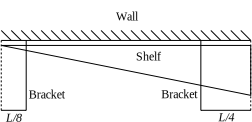
\includegraphics[width=0.4\textwidth]{../../../figures/Statics_triangle_shelf_question.svg}
	\caption{The new triangular shelf as seen from above}
	\label{fig:Statics_triangle_shelf_question}
\end{figure}}

\begin{enumerate}[resume]
	\item \question[b]{Find the new ratio of the forces on the two brackets.}
\end{enumerate}
  }
{The centre of mass of a triangle lies at a point $\frac{1}{3}$ of the perpendicular distance from the base to the tip.}
{\textit{Adapted with permission from UCLES, AO Level Physics, June 1989, Paper 1, Question 3}}
{\answer[a]{\valuedef{\frac{F_1}{F_2}}\frac{2}{3}{}}
\answer[b]{\valuedef{\frac{F_1}{F_2}}{\frac{2}{13}}}
\begin{enumerate}
	\item The centre of mass of the plank will be at its midpoint.
\begin{figure}[htbp]
	\centering
	\includegraphics[width=0.6\textwidth]{Statics_beam_reaction}
	\caption{The shelf with the contact forces from the brackets and all distances marked}
	\label{fig:Statics_beam_reaction}
\end{figure}

Considering moments about the centre of mass at equilibrium:
\begin{equation*}
r_1F_1-r_2F_2=0
\end{equation*}
From the diagram:
\begin{equation*}
r_1=\frac{L}{2}-\frac{L}{8}=\frac{3L}{8} 
\end{equation*}
\begin{equation*}
r_2=\frac{L}{2}-\frac{L}{4}=\frac{L}{4} 
\end{equation*}
\\
\begin{equation*}
\therefore \frac{3L}{8} \cdot F_1 = \frac{L}{4} \cdot F_2 
\end{equation*}
\begin{equation*} 
\frac{F_1}{F_2}=\frac{2}{3}
\end{equation*}
\\

	\item The centre of mass of a triangle is $\frac{1}{3}$ of the perpendicular distance from the base to the tip.
\begin{figure}[htbp]
	\centering
	\includegraphics[width=0.6\textwidth]{Statics_tri_beam_reaction}
	\caption{The triangular plank viewed side-on with the contact forces from the brackets and all distances marked}
	\label{fig:Statics_tri_beam_reaction}
\end{figure}

Taking moments about the centre of mass at equilibrium:
\begin{equation*}
r_1F_1-r_2F_2=0
\end{equation*}
From the diagram:
\begin{equation*}
r_1=\frac{2L}{3}-\frac{L}{8}=\frac{5L}{6} 
\end{equation*}
\begin{equation*}
r_2=\frac{L}{3}-\frac{L}{4}=\frac{L}{12} 
\end{equation*}
\\
\begin{equation*}
\therefore \frac{5L}{6} \cdot F_1 = \frac{L}{12} \cdot F_2 
\end{equation*}
\begin{equation*} 
\frac{F_1}{F_2}=\frac{2}{13}
\end{equation*}


\end{enumerate}
}
\end{hint}